% !XeLaTeX root=_main_.tex
% chapter2

\chapter{مفاهیم اولیه}\label{chapter2}
\thispagestyle{empty}

\epigraph{
	«آزمون نرم‌افزار می‌تواند وجود خطاها را نشان دهد، اما هرگز نمی‌تواند نبود آنها را تضمین کند.»
}
{$ \maltese $ {\large ادسـخر دایکـسترا}}


\noindent
در بخش اول این فصل تعاریف پایه‌ای آزمون نرم‌افزار و معیارهای سنجش آزمون، روش اندازه‌گیری و گزارش آنها را بیان می‌کنیم.
در بخش دوم، آزمون فازی، فنون مختلف به‌کار گرفته شده در این آزمون، آزمون فازی قالب فایل، روش‌های تولید خودکار داده آزمون در \gls{Fuzzer}ها و معماری فازرها را توضیح می‌دهیم. بخش سوم و چهارم را به معرفی فنون \gls{DeepLearning} و استفاده از آنها در وظایف یادگیری مبتنی بر \gls{Sequence} تخصیص داده‌ایم. در پایان نیز خلاصه‌ای از مطالب مطرح شده در فصل را می‌آوریم. مفاهیم اولیه بسیار گسترده‌تر از آنچه در این فصل مطرح گردیده هستند و به‌همین دلیل در بخش پایانی خواننده را به منابع مناسبی ارجاع داده‌ایم. همچنین مطالعه کامل‌تری در باب مطالب این فصل در گزارش سمینار کارشناسی ارشد اینجانب 
\cite{ZakeriSeminar2017}
انجام شده است.  



\section{آزمون نرم‌افزار}\label{software_testing}
مجموعه فنون کشف و آشکارسازی خرابی‌های نرم‌افزار در مراحل مختلف توسعه آن را
\textbf{آزمون نرم‌افزار}
گویند. منظور از خرابی بروز رفتار(های) ناخواسته و خلاف \gls{Specification}ها در یک نرم‌افزار یا قسمتی از آن است. خرابی خود حاصل یک خطا (نقص) ایستا در نرم‌افزار است. حالت داخلی نادرست برنامه را که ناشی از یک خطا است،  \gls{Error} می‌گویند
 \cite{ammann2016introduction}. واژه‌های خطا، اشکال و خرابی از حوزه \gls{Dependability} وارد آزمون نرم‌افزار شده‌اند
  \cite{Dubrova:2013:FD:2462571} و تعاریف یکسانی برای آنها وجود ندارد
  \cite{PaulC.Jorgensen2014,ammann2016introduction}.
  
  
  آزمون نرم‌افزار منحصر به کد اجرایی برنامه نیست و شامل آزمون \gls{Requirement}ها، آزمون مشخصه‌ها و \gls{Design} نیز می‌گردد. در آزمون فازی اما مُنحصراً به کد اجرایی پرداخته می‌شود. لذا در ادامه این پایان‌نامه، منظور از آزمون، فقط آزمون مربوط به کداجرایی برنامه خواهد بود. واژگان حاکم بر حوزه آزمون نرم‌افزار بسیار گسترده می‌باشد. در اینجا روی برخی از مفاهیم پایه‌ای‌ و مرتبط با آزمون فازی و تولید داده آزمون تمرکز می‌کنیم.
 
 \subsection{معیارهای پوشش}
  متأسفانه آزمون تنها قادر است وجود خرابی را نشان دهد و نبود آن را تضمین نمی‌کند. به‌بیان صوری، مسئله یافتن تمامی خرابی‌ها در یک برنامه \gls{Undecidable} است \cite{ammann2016introduction}. این موضوع سبب می‌شود به‌دنبال راه‌کارهایی برای اندازه‌گیری آزمون و تعیین میزان خوب بودن آن باشیم. در دهه‌های اخیر تمرکز بر روی \gls{CoverageCriteria}، شناسایی، تفکیک و سنجش آنها بوده است. معیارهای پوشش بیشتر با هدف کمی‌سازی و اندازه‌گیری مقدار آزمون انجام شده مطرح شده‌اند؛ هرچند متقابلاً در تولید داده آزمون هم کاربرد دارند. چون با مسئله‌ای \gls{Undecidable} مواجه هستیم، بایستی معیاری وجود داشته باشد که مشخص کند چه زمانی می‌توانیم آزمون را خاتمه دهیم و در این زمان آزمون تا چه‌حد خوب انجام شده است. آمان  \LTRfootnote{P.Ammann (\href{https://cs.gmu.edu/~pammann/}{https://cs.gmu.edu/~pammann})}
  	 و آفوت\LTRfootnote{J. Offutt (\href{https://cs.gmu.edu/~offutt/}{https://cs.gmu.edu/~offutt/})} \cite{ammann2016introduction}
  	   معیارهای پوشش را به‌صورت چهار معیار \gls{InputSpacePartitioning}،  \gls{GraphCoverage}، \gls{LogicCoverage}و \gls{SyntaxBasedCoverage} مطرح کرده‌اند.
  
  
  پوشش گراف در سطح کد اجرایی که به آن پوشش کد هم گفته می‌شود، شامل پوشش گراف جریان کنترل (\gls{CFG}) و گراف جریان داده (\gls{DFG}) برنامه می‌شود. پوشش  منطق، مقدار‌دهی و تعیین ارزش عبارات منطقی ظاهر شده در متن برنامه است. افراز فضای ورودی یعنی انتخاب از بین حالت‌های مختلف ترکیب ورودی‌ها و در نهایت پوشش ساختار نحوی، استفاده از قوانین گرامر برای \gls{Validation} داده‌های ورودی یا تولید داده‌های جدید آزمون را شامل می‌شود.
  
  
  معیارهای پوشش به دو روش مختلف قابل استفاده هستند. یک روش به این صورت است که مقادیر داده‌های آزمون منحصراً برای برآوردن یک معیار داده شده، تولید گردند. این روش در برخی موارد بسیار دشوار است. به‌ویژه اگر ابزاری برای تولید خودکار داده آزمون نداشته باشیم یا ساختار ورودی پیچیده باشد. روش دوم تولید داده‌های آزمون به‌طور کاملاً مجزا و سپس اندازه‌گیری میزان پوشش معیار مربوطه است. برای روش اول یک \gls{RecognizerProgram} برآورده شدن معیار و برای روش دوم یک \gls{GeneratorProgram} داده آزمون نیاز است. در صنعت استفاده از روش دوم مرسوم‌تر است\cite{ammann2016introduction}.
  
  
  در این پایان‌نامه، معیار دوم از معیارهای پوشش (پوشش کد) با روش دوم را مبنا قرار می‌دهیم. به این صورت که یک روش تولید خودکار داده آزمون و اندازه‌گیری میزان پوشش کد ارایه خواهیم داد. این فن آزمون، به‌خوبی عملی بوده و آزمون فازی معمول نیز بر اساس این روش است. پوشش کد خود در سطوح مختلفی مطرح است؛ \gls{StatementCoverage}، \gls{BranchCoverage} و \gls{PathCoverage} سه سطح شناخته شده هستند. در پوشش دستور اجرای حداقل یک‌مرتبه هر دستور برنامه به عنوان نیازمندی تعریف و سپس اندازه‌گیری می‌شود. در پوشش شاخه اجرای حداقل یک‌مرتبه هر انشعاب برنامه به عنوان نیازمندی مطرح است و بلأخره در پوشش مسیر اجرای حداقل یک‌مرتبه هر مسیر اجرایی مد نظر است. بدیهی است که  پوشش مسیر، پوشش شاخه و پوشش شاخه، پوشش دستور را شامل می‌شود. تعاریف و فهرست کاملی از سطوح پوشش کد و رابطه بین آنها در \cite{ammann2016introduction} ذکر شده است. 
  
  شرکت مایکروسافت در محیط توسعه مجتمع ویژوال استادیو\LTRfootnote{Visual Studio (\href{https://visualstudio.microsoft.com/}{visualstudio.microsoft.com})}، معیارهای  \gls{LineCoverage}، \gls{BasicBlockCoverage} و \gls{PartialLineCoverage} را ارایه کرده است. \gls{LineCoverage} همان پوشش دستور در کد سطح بالا (به‌جای کد اسمبلی/ماشین) است. \gls{BasicBlockCoverage} تعمیمی از پوشش دستور است که در آن یک توالی از دستورهای برنامه که شامل هیچ دستور پرشی در بین خود نیستند، یک دستور واحد در نظر گرفته ‌می‌شوند. مزیت پوشش کد در سطح دستور و \gls{BasicBlock} سادگی اندازه‌گیری آن و عدم نیاز به وجود \gls{SourceCode} برنامه است \cite{Dubrova:2013:FD:2462571}. پوشش خط جزئی منظور اجرا شدن برخی از قسمت‌های یک خط کد سطح بالا است. برای مثال در خطوطی با عبارات شرطی طولانی بر اثر ارزیابی مدار کوتاه  \LTRfootnote{\lr{Short-Circuit Evaluation}}
   ممکن است کلیه دستورات آن خط کد اجرا نگردد. در نتیجه پوشش خط جزئی معیاری متفاوت از پوشش خط است.
  
  
  علاوه بر موارد ذکر شده معیارهای دیگری هم برای پوشش کد ارایه گردیده، از جمله \gls{DomainCoverage} که در \textbf{آزمایشگاه تحقیقاتی \gls{ReverseEngineering} دانشگاه علم و صنعت ایران}
  \LTRfootnote{IUST Reverse Engineering Research Laboratory (\href{http://parsa.iust.ac.ir/reverse-engineering-lab/}{http://parsa.iust.ac.ir/reverse-engineering-lab/}) } 
توسعه داده شده است \cite{Nikravan2018}. پوشش دامنه، نوعی از معیار افراز فضای حالت 
\cite{ammann2016introduction}
است که در آن با استناد به تئـوری مجموعه‌ها، دامنه‌هایی برای هریک از ورودی‌های برنامه تعیین می‌شود. انتخاب ورودی از این دامنه‌ها در زمان آزمون، منجربه پوشش یک مسیر مشخص شده می‌گردد. از آنجایی که تنها یک بار اجرای یک مسیر، لزوماً خطای موجود در آن را آشکار نمی‌کند؛ در این روش می‌توان مسیر داده‌ شده را به هر تعداد و هر بار با داده‌های آزمون متفاوت  آزمون کرد. از این دیدگاه، پوشش دامنه یک روش تولید داده آزمون را ارایه می‌دهد.

در این پایان‌نامه، \gls{BasicBlockCoverage} و \gls{LineCoverage}  را برای گزارش میزان پوشش کد به کار می‌بریم. در بین این دو معیار، پوشش بلوک پایه در مقایسه با پوشش خط برنامه معیار مناسب‌تری است؛ زیرا، تعداد خطوط برنامه را می‌توان تغییر داد. برای مثال چندین دستور را در یک خط قرار داد یا اینکه یک دستور را در چند خط نوشت. تعداد بلوک پایه اما مستقل از نحوه آرایش و قرارگیری خطوط برنامه است و این معیار با تغییراتی مانند آنچه گفته شد، تغییر نمی‌کند؛ زیرا، در هر حالت تعداد بلوک‌های پایه یک برنامه و گراف جریان کنترل ثابت است. البته این تأکید صرفاً برای مواردی است که ممکن است آرایش خطوط برنامه در آزمون‌های مختلف تغییر کند، بدون اینکه تغییری در خود کد ایجاد شده باشد.
  
  
  
  \subsection{دیدگاه جعبه}\label{box_view}
  نحوه اندازه‌گیری معیارهای بحث شده، تنظیم و سنجش آزمون، منوط به اطلاعات در دسترس از \gls{SUT} است. آزمون نرم‌افزار را براساس اطلاعات در دسترس از \gls{SUT} در زمان آزمون، به سـه دسته/ حالت \gls{BlackBox}، \gls{WhiteBox} و \gls{GrayBox} تقسیم‌بندی می‌کنند \cite{ammann2016introduction,Mcnally2012}، که آن ‌را دیدگاه جعبه به آزمون نرم‌افزار گوییم. شکل \ref{ch2_box_veiw_test_triangle_crop.pdf} این تقسیم‌بندی را به‌صورت یک طرح‌واره مثلثی نشان می‌دهد.
  %https://pdfresizer.com/crop/ea1df3dc10.pdf
  \begin{figure}%[tbh!]%[ht]%[t!]
  	\centering
  	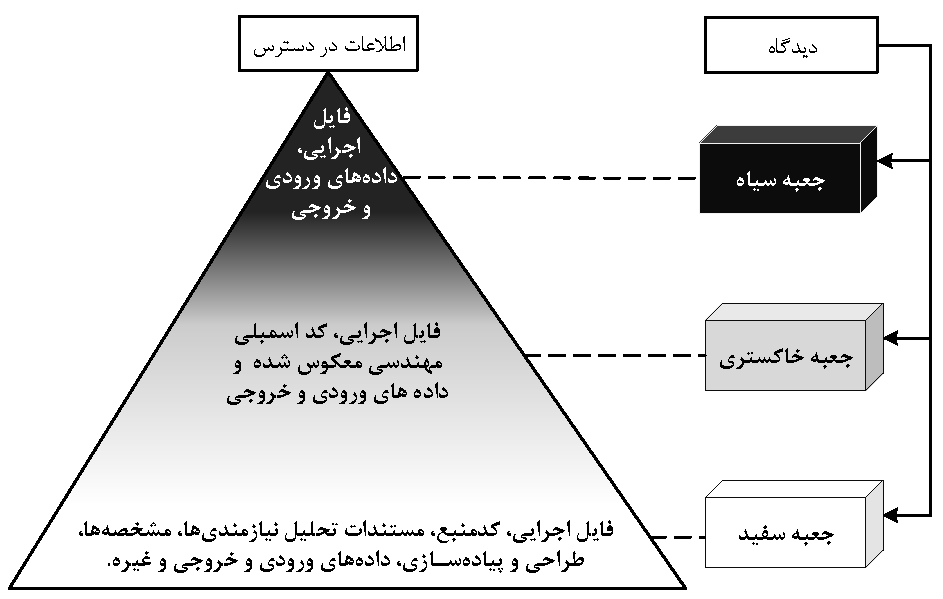
\includegraphics[width=\textwidth, clip=true,  trim= 0 0 0 0]{chapter2/ch2_box_veiw_test_triangle_crop.pdf}
  	%\includegraphics[width=\textwidth]{figs/chapter1/ch1_fuzz_testing_flowchart2.png}
  	\caption[دیدگاه جعبه در آزمون نرم‌افزار]
  	{
  		طرح‌واره‌ای از دیدگاه جعبه بر اساس اطلاعات در دسترس به‌صورت یک مثلث آزمون\cite{ZakeriSeminar2017}.
  	}
  	\label{ch2_box_veiw_test_triangle_crop.pdf}
  \end{figure}
  
  
  همان‌طور که در این طرح‌واره پیداست، در رأس مثلث، هیچ اطلاعی از ساختار داخلی \gls{SUT} در اختیار آزمون‌گر نیست. در واقع با برنامه به مثابه یک جعبه سیاه که ورودی را دریافت و خروجی تولید می‌کند، رفتار می‌شود. این نوع آزمون معمولاً روی برنامه‌هایی که منتشر شده‌اند و توسط افرادی خارج از تیم توسعه و پشتیبانی محصول انجام می‌شود. هدف آن هم بیشتر کشف آسیب‌پذیری‌‌ها و ضعف‌های امنیتی است. در پایین مثلث، دیدگاه جعبه سفید وجود دارد. در اینجا تقریباً تمامی اطلاعات \gls{SUT} در دسترس است. دیدگاه جعبه خاکستری مابین دو دیدگاه قبلی قرار دارد. در این دیدگاه از فنون مهندسی معکوس برای استخراج اطلاعات از \gls{SUT} استفاده می‌شود. هریک از این دیدگاه‌ها مزایا و معایب خاص خود را دارند\cite{Khan2012}. آزمون فازی هم که در ادامه مطرح می‌شود، قابل تقسیم به‌این سه دسته است. آزمون فازی جعبه خاکستری، برای مثال، بسیار ثمربخش بوده است   \cite{DBLP:journals/corr/abs-1711-04596, Zalewsky2013}. روش پیشنهادی در این پایان‌نامه برای تولید داده آزمون، قابل استفاده در هر سه دسته آزمون فازی است. برای ارزیابی روش پیشنهادی در این پایان‌نامه، در \hyperref[ch:5]{فصـل 5}، اما از آزمون جعبه سفید، استفاده کرده‌ایم تا بتوانیم معیارهای پوشش کد و بخش‌های اجرا شده را به‌دقت اندازه‌گیری نماییم. از طرفی \lr{SUT} انتخابی ما متن باز و رایگان بوده و در این حالت کد منبع آن دردسترس است. 
 
     
  \subsection{اندازه‌گیری پوشش کد}\label{sec:instrumenting}
   هدف از مطرح کردن دیدگاه جعبه در بخش \ref{box_view}، اشاره به امکانات لازم برای اندازه‌گیری معیارهای پوشش از جمله پوشش کد بود. در آزمون جعبه سفید که کد منبع برنامه وجود دارد، مشاهده پوشش کد برنامه با اضافه کردن دستوراتی به متن کد به آسانی امکان پذیر است. این عمل را \gls{Instrumenting} کد یا تجهیز برنامه به کد رهگیری می‌نامند\cite{Rathaus:2007:OSF:1536880}. در محیط \lr{GNU/GCC} (زبان‌های \lr{C} و \lr{C++})، برای \gls{Instrumenting} کافی است کد منبع برنامه را همراه با پرچم‌های
   \lr{\texttt{-fprofile-arcs}}
   و
   \lr{\texttt{-ftest-coverage}}
   کامپایل کنیم:\\
   
   
   \begin{LTR}
   	\begin{lstlisting}[language=bash, caption={\rl{ابزارگذاری کد در محیط \lr{GNU/GCC}.}}, label={codesnip2}]
   	~$ gcc -g -fprofile-arcs -ftest-coverage -o test test.c
   	~$ ./test f1 f2
   	~$ gcov test.c
   	~$ more test.c.gcov\end{lstlisting}
   \end{LTR}
سطر اول برنامه \ref{codesnip2} برنامه \lr{test} را با پرچم‌های ذکر شده کامپایل می‌کند. سطر دوم برنامه را با دو آرگومان خط فرمان \texttt{f1} و \texttt{f2} اجرا می‌کند. سطر سوم پوشش کد اجرای اخیر برنامه را محاسبه و فایلی تحت عنوان \texttt{ test.c.gcov} تولید می‌کند. در سطر چهارم این فایل برای مشاهده باز می‌شود. افزون بر این، پرچم‌هایی برای اخذ انواع سطوح پوشش کدی که بحث شد، از جمله پوشش شاخه، وجود دارد \cite{Rathaus:2007:OSF:1536880}. 

  محیط ویژوال استادیو ابزار \lr{vsinstr} را برای ابزارگذاری کد برنامه و \lr{VSPerfMon} را برای اندازه‌گیری پوشش کدِ زبان‌های پشتیبانی شده توسط این محیط، ارائه می‌دهد که البته در حضور کد منبع برنامه قابل استفاده هستند. هنگامی که کد منبع در اختیار نباشد کار اندکی دشوار می‌شود. در این موارد، بایستی از ابزارهای مهندسی معکوس و ابزارگذاری کد باینری استفاده کرد.
 \lr{DynamoRIO}\LTRfootnote{\href{http://www.dynamorio.org/}{http://www.dynamorio.org/}}\cite{Bruening:2004:ETC:1087758}،
 \lr{Pin}\LTRfootnote{\href{https://software.intel.com/en-us/articles/pin-a-dynamic-binary-instrumentation-tool}{https://software.intel.com/en-us/articles/pin-a-dynamic-binary-instrumentation-tool}}\cite{Luk:2005:PBC:1064978.1065034}،
 \lr{PaiMei}\LTRfootnote{\href{https://github.com/OpenRCE/paimei}{https://github.com/OpenRCE/paimei}}\cite{Rathaus:2007:OSF:1536880}
  و 
  \lr{QEMU}\LTRfootnote{\href{https://www.qemu.org/}{https://www.qemu.org/}} \cite{QEMU2018}
 ابزارهایی برای این منظور فراهم کرده‌اند.


  
\section{آزمون فازی}
\gls{FuzzTesting}\cite{Miller:1990:ESR:96267.96279,Miller1995,Forrester:2000:ESR:1267102.1267108,Miller:2006:ESR:1145735.1145743}
همان‌طورکه قبلاً هم گفتیم، فرایند ساده تولید و سپس تزریق یک ورودی ناخواسته (بدشکل شده یا نامتعارف) به \gls{SUT} است. چنان‌چه برنامه بر اثر پردازش این ورودی ناخواسته دچار خرابی شود، حافظه برنامه مورد تحلیل قرار گرفته و خطای احتمالی موجود در کد آشکار می‌گردد. به دلیل اینکه \gls{SUT} هنگام آزمون اجرا می‌شود، آزمون فازی، نوعی آزمون پویا است. چون \gls{SUT} با تعداد ورودی‌های بسیار زیادی مورد آزمون قرار می‌گیرد، آزمون فازی را می‌توان نوعی\gls{StressTesting} هم به‌شمار آورد. فرایند معمول آزمون فازی در ‏شکل
\ref{ch2_fuzz_testing_flowchart_crop.pdf} نشان داده شده است.


%% Need to crop all figures
%% https://pdfresizer.com/
%%
\begin{figure}%[tbh!]%[ht]%[t!]
	\centering
	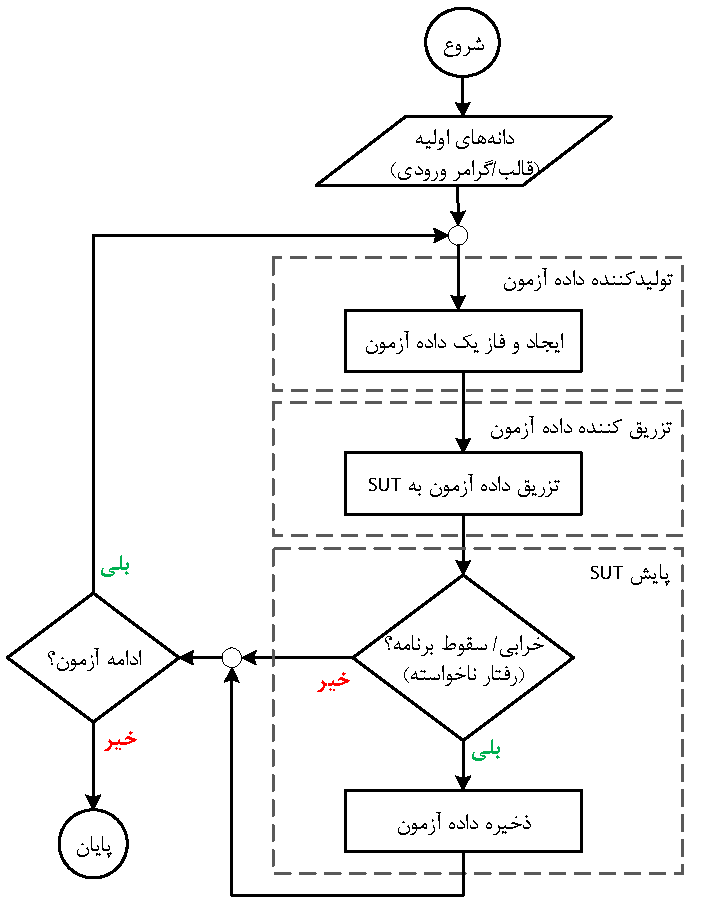
\includegraphics[width=0.9\textwidth, clip=true,  trim= 0 0 0 0]{chapter2/ch2_fuzz_testing_flowchart_crop.pdf}
	%\includegraphics[width=\textwidth]{figs/chapter1/ch1_fuzz_testing_flowchart2.png}
	\caption[روندنمای  فرایند آزمون فازی]
	{
		روندنمای فرایند آزمون فازی در حالت ساده که با اقتباس از مراجع مختلف ترسیم شده است. پیمانه‌های مورد نیاز برای خودکارسازی فرایند با مستطیل خطچین مشخص شده‌اند. شرایط ادامه آزمون می‌تواند بر عهده فرد آزمون‌گر قرار داده شود یا توسط خود فازر تعیین گردد.
	}
	\label{ch2_fuzz_testing_flowchart_crop.pdf}
\end{figure}



\subsection{فازر}\label{sec:fuzzer}
\gls{Fuzzer} ابزاری است که فرایند آزمون فازی را خودکار می‌کند. پیاده‌سازی هریک از \gls{Module}‌های شکل
\ref{ch2_fuzz_testing_flowchart_crop.pdf}
و تجمیع آنها در کنار یکدیگر یک \gls{Fuzzer} را ایجاد می‌کند. تمرکز اصلی در یک \gls{Fuzzer}، نحوه تولید ورودی جدید به عنوان داده آزمون است به‌گونه‌ای که می‌توان آن را وجه تمایز اصلی فازرهای مختلف دانست. روش‌های تولید داده در فازرها قابل تفکیک به دو دسته کلی روش‌های \gls{MutationBased} یا جهش و روش‌های \gls{GenerationBased} 
هستند \cite{Chen2018}.


در روش \gls{MutationBased}، تعداد یک یا بیشتر داده ورودی \gls{Valid} به‌عنوان \gls{InitialSeed} برای تولید داده‌های آزمون بیشتر به‌کار می‌رود.  \gls{InitialSeed} جهش (تغییر ناگهانی) می‌یابد تا داده آزمون دیگری تولید شود. جهش می‌تواند ساده باشد؛ شبیه معکوس کردن یک بیت، جایگزین کردن یک کاراکتر، یا پیچیده‌تر باشد؛ شبیه شناسایی و تکرار ساختارهای مشخص در داده، جایگزینی اعداد صحیح و حقیقی با مقادیر مرزی (بسیار بزرگ یا کوچک) و غیره. ساختن یک فازر مبتنی بر جابه‌جایی و تولید ورودی بد شکل و مخرب با آن، آسان است و نیاز به شناخت قبلی ساختار داده ورودی مورد جهش ندارد. عیب روش مبتنی بر جابه‌جایی اینجاست که این روش وابسته به تنوع ورودی‌های نمونه است. بدون وجود ورودی‌های مختلف با پیچیدگی کافی، این نوع فارز‌ به پوشش کد بالایی دست نمی‌یابد \cite{Kettunen2014}. به عبارت دیگر دانه اولیه در فازر مبتنی بر جابه‌جایی بسیار حائز اهمیت است.
 \lr{AFL}\LTRfootnote{American Fuzzy Lop (\href{http://lcamtuf.coredump.cx/afl/}{http://lcamtuf.coredump.cx/afl/})}\cite{Zalewsky2013}، \lr{FileFuzz}\LTRfootnote{\href{http://www.fuzzing.org/}{http://www.fuzzing.org/}}\cite{Sutton:2007:FBF:1324770}
 و
  \lr{Radamsa}\LTRfootnote{\href{https://gitlab.com/akihe/radamsa}{https://gitlab.com/akihe/radamsa}}\cite{Kettunen2014}
 نمونه‌هایی از فــازرهای مبتنی بر جابه‌جایی هستند.
 
 
 روش مبتنی بر تولید، داده‌های آزمون را به‌صورت کاملاً تصادفی یا از روی یک توصیف صوری مانند گرامر، قالب، یا مدل تولید می‌کند. در حالت دوم، از مشخصه‌های داده ورودی، برای ساخت یک \gls{GenerativeModel} استفاده می‌شود. این روش بیشتر روی قالب‌های داده‌ای که مستنداتی از مشخه‌های آنها در دسترس است، به‌کار می‌رود که در مقایسه با فازرهای مبتنی بر جابه‌جایی، معمولاً به پوشش کد بالاتری دست می‌یابد. با این حال، همان‌طور که در فصل 1 هم اشاره شد، زمان و هزینه زیادی باید صرف شود تا مشخصه‌های یک قالب داده، کامل فهمیده و مدل خوبی از آن تهیه شود؛ زیرا، این کار تمام خودکار نیست \cite{Miller2007} و از طرفی، مستندات ساختار ورودی همواره در دسترس آزمون‌گر، نیستند.
 SPIKEfile\LTRfootnote{\href{http://fuzzing.org/}{http://fuzzing.org/}}\cite{Sutton:2007:FBF:1324770} و
 Peach\LTRfootnote{\href{https://www.peach.tech/}{https://www.peach.tech/}}
 نمونه‌ای از فازرهای مبتنی بر تولید هستند. روش‌های ترکیبی نیز وجود دارد که از ویژگی‌های هر دو روش بیان شده در تولید مورد آزمون کمک می‌گیرد. یک مثال از فازرهای ترکیبی LangFuzz \cite{Holler2012} است.
 
 
 \subsection{معماری فازرها}\label{sec:fuzzers_architechture}
 یک معماری مرجع برای فازرها وجود ندارد؛ ولی می‌توان از روی فرایند ترسیم شده برای آزمون فازی (شکل  \ref{ch2_fuzz_testing_flowchart_crop.pdf})، پیمانه‌های اصلی لازم برای یک فازر را پیشنهاد کرد. پیمانه اول تولید کننده \gls{TestData}است که داده‌های ورودی لازم برای آزمون را تولید می‌کند. دیدیم که روش‌های مختلفی برای تولید داده آزمون وجود دارند. پیمانه دوم تزریق کننده داده آزمون است که وظیفه آن تحویل داده‌های تولید شده توسط تولیدکننده به \gls{SUT} است. هر برنامه واسط مختص به خود را دارد. واسط می‌تواند \gls{CLI}، گرافیکی (\gls{GUI})، پروتکل شبکه یا فایل باشد. هدف این پایان‌نامه برنامه‌هایی هستند که ورودی آنها فایل است. معمولاً داده‌های ورودی به‌شکل فایل (مثل \gls{PDF}) ساختار پیچیده‌تری نسبت به داده‌های \gls{CLI} و پروتکل‌های شبکه دارند و تولید آنها سخت‌تر است. فازری که برای آزمون این برنامه‌ها توسعه داده می‌شود، \gls{FileFormatFuzzer} هم نامیده می‌شود \cite{Sutton:2007:FBF:1324770}.
 
 
 آخرین پیمانه مورد نیاز ابزار یا محیط پایش است که \gls{SUT} را پایش می‌کند تا در صورت بروز خرابی ضمن ذخیره حالت برنامه، محل وقوع خرابی را بتواند با تحلیل حافظه برنامه مشخص کند. البته ابزارهای مستقل زیادی برای این منظور وجود دارند که می‌توان از آنها بهره گرفت. 
 \lr{Application Verifier}\LTRfootnote{\href{https://docs.microsoft.com/en-us/windows-hardware/drivers/debugger/application-verifier}{https://docs.microsoft.com/en-us/windows-hardware/drivers/debugger/application-verifier}}
 \cite{ApplicationVerifier}
 یک ابزار پایشِ قابل استفاده در سیستم عامل ویندوز است. ممکن است فازر، یک بازخورد از ابزار پایش برای تولید داده آزمون بعدی دریافت کند. این بازخورد عموماً حاوی اطلاعات مربوط به پوشش کد اجرای برنامه است. بر این اساس فازرها به دو دسته دارای حلقه بازخورد و بدون حلقه بازخورد تقسیم‌بندی می‌شوند \cite{Chen2018}.
 AFL\cite{Zalewsky2013}
 یک فازر دارای حلقه بازخورد است. در این پایان‌نامه یک فازر ساده قالب فایل بدون حلقه بازخورد ارائه می‌دهیم. تمرکز برروی نحوه تولید داده آزمون به روش \gls{GenerationBased} / گرامر است.
 
 
 
 \subsection{آسیب‌پذیری}
 آزمون فازی می‌تواند برای اهداف مختلفی استفاده شود، اما مهمترین هدف آن تحلیل نرم‌افزار به منظور کشف آسیب‌پذیری‌ها است. یعنی می‌توان آن را نوعی \gls{PenetrationTesting}، \gls{RobustnessTesting} و \gls{SecurityTesting} هم تعریف کرد. تعاریف گوناگونی برای اصطلاح آسیب‌پذیری نرم‌افزار وجود دارد. آسیب‌پذیری را می‌توان اجتماع سه عنــصر دانست: وجود یک خطا در نرم‌افزار، دسترسی مهاجم به خطا و قابلیت مهاجم برای \gls{Exploit} از خطا \cite{Chen2018,InternetSecurityGlossary}. چنانچه پیش از این اشاره شد، خطا، نرم‌افزار را در یک حالت اشکال قرار می‌دهد که منجربه خرابی می‌شود. بعضی خطاها ممکن است تنها منجربه خرابی نرم‌افزار و بروز رفتار ناخواسته (مغایر با مشخصه‌ها) شوند. بنابراین صرف وجود یک خطا در نرم‌افزار آسیب‌پذیری محسوب نمی‌گردد 
 \cite{Sutton:2007:FBF:1324770,Rathaus:2007:OSF:1536880}.
 
 
 انواع مختلفی از خطاها وجود دارند که می‌توانند توسط فازرها کشف شوند؛ به‌ویژه آنهایی که از جنس نقض دسترسی به حافظه هستند. خطاهای فساد حافظه بدون شک رایج‌ترین و مؤثرترین روش بهره‌برداری خرابکارانه از یک سیستم کامپیوتری محلی یا راه دور هستند. اگر حافظه بتواند به روشی خراب شود (یک آدرس بازگشت، یک اشاره‌گر پشته، یک اشاره‌گر تابع و غیره) اغلب اجرا می‌تواند به کد تهیه شده توسط مهاجم هدایت شود. بیشترین آسیب‌پذیری‌هایی که معمولاً توسط محققین حوزه امنیت کشف می‌شوند، مرتبط با \gls{Buffer} (یک ناحیه ثابت از حافظه اصلی در اختیار برنامه) هستند؛ از جمله سرریز میانگیر، سرریز پشته، سرریز عدد صحیح و غیره \cite{Takanen:2008:FSS:1404500}. در آزمون فازی به‌دنبال یافتن چنین خطاهایی از طریق تزریق ورودی بدشکل و خرابی حافظه \gls{SUT} هستیم. مطالعه و طبقه‌بندی کاملی از انواع آسیب‌پذیری‌ها در \cite{ZakeriSeminar2017} انجام شده است.  
 
 
 
 
 %%%%%%%%%%%%%%%%%%%%%%%%%%%%%%%
 %%%  Deep Learning Section  %%%
 %%%%%%%%%%%%%%%%%%%%%%%%%%%%%%%
 
 \section{یادگـیری ژرف}
  \gls{DeepLearning}
مجموعه‌ای از فنون یادگیری ماشینی است که در آن بردار ویژگی‌ها به‌صورت خودکار از داده‌های خام استخراج می‌گردد. ابزار اصلی و غالب در این فنون از یادگیری،  \glspl{NeuralNetwork} هستند. در حالت ساده \glspl{NeuralNetwork} به مسئله یک تابع را نسبت داده و آن را مدل می‌کند. پارامترهای این تابع سپس در فرایند آموزش مدل، تخمین زده می‌شوند. در \gls{DeepLearning} تعداد این پارامترها صدها، هزارها و گاهی میلیون‌ها برابر افزایش می‌یابد که در نتیجه قدرت  \gls{Representation} و حل مسئله مدل، افزایش خواهد یافت. شبکه عصبی در این حالت یک گراف با ژرفای بیش از یک یال، خواهد بود که به آن \gls{DeepNeuralNetwork} هم می‌گویند. شبکه عصبی ژرف بدین ترتیب قادر به استخراج و تمییز جزئی‌ترین ویژگی‌های مسئله و در نتیجه بهبود دقت حاصله، خواهد بود \cite{Goodfellow-et-al-2016}.
 
 
 وجود تعداد بسیاری پارامتر در مدل‌های یادگیری ژرف، سبب می‌شود که آموزش این مدل‌ها از لحاظ محاسباتی سنگین و زمان‌بر باشد. بسیاری از موانع تئوری و عملی آموزش این مدل‌ها به‌تازگی رفع شده‌اند. برای مسائل مختلف، مدل‌های متفاوتی با شبکه‌های عصبی ژرف طراحی و ساخته می‌شوند. \gls{FeedforwardNeuralNetwork} ساده‌ترین نوع است. شبکه عصبی پیچشی (\gls{CNN}) مناسب وظایف بینایی ماشین و شبکه عصبی مکرر (\gls{RNN}) مناسب وظایف پردازش زبان طبیعی (\gls{NLP}) (وظایف مبتنی بر \gls{Sequence}) ایجاد شده‌اند. وجه مشترک همه شبکه‌های نام‌برده، بلوک سازنده آن یعنی \gls{Neuron} است \cite{Jurafsky2017}. 
 
 
 
 \subsection{عصب}
 بلوک محاسباتی پایه در بستر شبکه‌های عصبی، \gls{Neuron} یا \gls{Unit} است. یک عصب تعدادی عدد حقیقی را به‌عنوان ورودی گرفته، محاسباتی روی آنها انجام داده و یک خروجی تولید می‌کند. محاسبه بدین صورت است که عصب جمع وزن‌دار ورودی‌هایی که به آن وارد می‌شوند را به همراه یک مقدار اضافی به عنوان \gls{Bias} حساب می‌کند. سپس برای جلوگیری از محدود شدن فضای توابع قابل تخمین به فضایی خطی، یک تابع غیرخطی، موسوم به \gls{ActivationFunction} (تابع فعّالیت)، روی حاصل جمع اعمال می‌شود. توابع انگیزش متداول عبارتند از \lr{sigmoid} و \lr{tanh}. شکل \ref{ch2_single_neuron_internal_structure_crop.pdf} ساختمان داخلی یک عصب تنها با ورودی‌های $x_1 $، $ x_2 $ و $ x_3 $، متقابلاً وزن‌های $ w_1 $، $ w_2 $ و $ w_3 $ و مقدار بایاس $ b $ را نشان می‌دهد. محاسبات این عصب مطابق رابطه‌های \ref{NeuronActivation} و \ref{NeuronActivation2} است.
 \begin{equation}\label{NeuronActivation}
 z = b+ \sum_iw_ix_i 
 \end{equation}
 \begin{equation}\label{NeuronActivation2}
 y = \sigma(z)
 \end{equation}
 
 
 رابطه \ref{NeuronActivation} را می‌توان به صورت ضرب داخلی بردارهای $ W $ و $ x $ هم نشان داد که نمایش مرسوم‌تری است \cite{Jurafsky2017}:
  \begin{equation}\label{NeuronActivation3}
 z = b+ W.x
 \end{equation} 
 
 
 \begin{figure}%[ht!]%[tbh!]%[ht]%[t!]
 	\centering
 	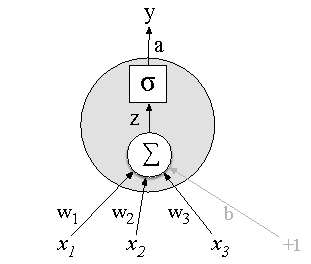
\includegraphics[width=0.5\textwidth, clip=true,  trim= 0 0 0 0]{chapter2/ch2_single_neuron_internal_structure_crop.pdf}
 	%\includegraphics[width=\textwidth]{figs/chapter1/ch1_fuzz_testing_flowchart2.png}
 	\caption[ساختمان داخلی یک عصب]
 	{
 		ساختمان داخلی یک عصب با ورودی‌های $x_1 $، $ x_2 $ و $ x_3 $، به‌ترتیب با وزن‌های $ w_1 $، $ w_2 $ و $ w_3 $، مقدار بایاس $ b $ و خروجی $y$ \cite{Jurafsky2017}.
 	}
 	\label{ch2_single_neuron_internal_structure_crop.pdf}
 	%\ref{ch2_single_neuron_internal_structure_crop.pdf}
 \end{figure}
 
 
 
 \subsection{شبکه عصبی روبه‌جلو}
 شبکه روبه‌جلو را می‌توان با یک گراف جهت‌دار بدون دور (\gls{DAG}) نشان‌ داد. هر گره یک عصب را نشان می‌دهد. گره‌هایی که مسیری به یکدیگر ندارند، یک لایه را تشکیل می‌دهند. ورودی هر لایه، خروجی عصب‌های لایه قبلی است. هر لایه بازنمایی یک \gls{Concept} در قالب یک تابع است و مسئله ترکیبی از این \glspl{Concept} است. یک شبکه با دو لایه تابع 
 $ f(x)=W_2\sigma(W_1 x) $
 را پیاده می‌کند که $ W_1 $ و $ W_2 $  ماتریس پارامترهای تابع و $ \sigma $ تابع انگیزش است.
 $ f(x)=W_3\sigma(W_2\sigma(W_1 x)) $
 معرف یک شبکه سه‌لایه خواهد بود. شکل \ref{ch2_feed_forward_neural_network_crop.pdf} دو گراف محاسباتی با ژرفای 2 و 3 لایه (به ترتیب از چپ به راست) را نشان می‌دهد. لایه‌های میانی را \glspl{HiddenLayer} هم می‌گویند. توجه شود که ورودی اول شبکه یک لایه محاسباتی نیست و بنابراین در شمارش لایه‌ها، شمرده نمی‌شود.
 
 
     
 \begin{figure}[ht!]%[tbh!]%[ht]%[t!]
 	\centering
 	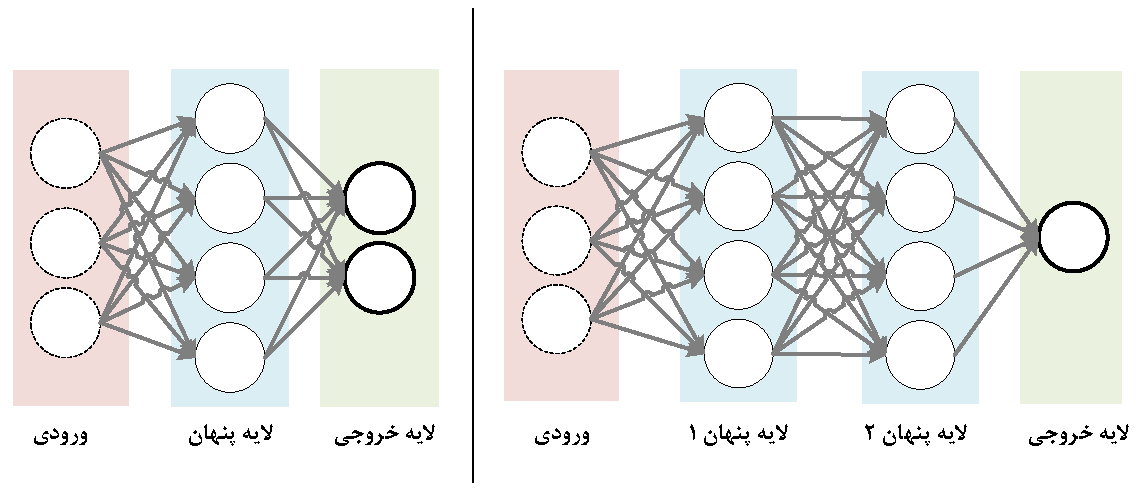
\includegraphics[width=\textwidth, clip=true,  trim= 0 0 0 0]{chapter2/ch2_feed_forward_neural_network_crop.pdf}
 	%\includegraphics[width=\textwidth]{figs/chapter1/ch1_fuzz_testing_flowchart2.png}
 	\caption[گراف محاسباتی شبکه عصبی روبه‌جلو]
 	{
 		گراف محاسباتی برای دو شبکه عصبی روبه‌جلوی فرضی. چپ: یک شبکه عصبی دو لایه (یک لایه پنهان متشکل از چهار عصب و یک لایه خروجی متشکل از دو عصب) به‌همراه سه ورودی. راست: یک شبکه عصبی سه‌لایه (دو لایه پنهان هر کدام متشکل از چهار عصب و یک لایه خروجی متشکل از یک عصب) و به‌همراه سه ورودی. 
 	}
 	\label{ch2_feed_forward_neural_network_crop.pdf}
 	%\ref{ch2_feed_forward_neural_network_crop.pdf}
 \end{figure}
 
 
 \subsection{آموزش شبکه روبه‌جلو}\label{feedforwardtraining}
 هدف از آموزش شبکه، تعیین مقادیر مناسب برای ضرایب و بایاس‌ها و سپس استفاده از شبکه برای انجام \gls{Task} مورد نظر است. داده‌هایی که در فرایند آموزش شبکه استفاده می‌گردد \gls{TrainingSet} نامیده می‌شوند. داده‌هایی که شبکه با آن مورد سنجش قرار می‌گیرد، \gls{TestSet} نامیده می‌شوند و مجموعه سوم از داده‌ها که در طول فرایند آموزش شبکه برای انتخاب بهترین راهکارهای یادگیری به‌کار گرفته می‌شوند، به نام \gls{ValidationSet} شناخته می‌شوند \cite{Goodfellow-et-al-2016}. 
 
 
 شبکه عصبی در یک راهبرد \gls{Supervised} آموزش می‌بیند. در \gls{SupervisedLearning} هر نمونه در مجموعه داده، علاوه بر بردار ویژگی‌ها با یک \gls{Label} همراه است که نقش ناظر را ایفا می‌کند. \gls{Classification} نمونه‌ای از وظایف \gls{SupervisedLearning} است. در این وظیفه برای هر ورودی، کلاس خروجی آن در زمان آموزش مشخص است.
 
 
 در فرایند آموزش ابتدا پارامترهای شبکه مقداردهی اولیه می‌شوند (معمولاً به‌صورت تصادفی). سپس به ازای هر ورودی از مجموعه آموزش، عصب‌های هر لایه خروجی خود را تولید می‌کنند تا زمانی که خروجی نهایی شبکه تولید شود. این مرحله را \gls{ForwardPass} می‌گویند. از آنجایی که خروجی درست برای ورودی مربوطه در زمان آموزش دردسترس است (\gls{SupervisedLearning})؛ اختلاف مقدار محاسبه شده توسط شبکه ($ \hat{y} $) و مقدار واقعی ($ y $)، توسط تابعی موسوم به \gls{ErrorFunction} یا \gls{CostFunction} یا تابع هدف محاسبه می‌شود \cite{Karpathy2016}. توابع مختلفی برای این منظور می‌توان تعریف کرد. 
 تابع \gls{MeanAbsoluteError} (رابطه \ref{MAELossFunction})، تابع \gls{MeanSquaredError} (رابطه \ref{MSELossFunction}) و تابع \gls{CrossEntropyError} (رابطه \ref{CrossEntropyLossFunction}) توابعی هستند که بسته به وظیفه مورد نظر استفاده می‌شوند \cite{Sautermeister2016}.
\begin{equation}\label{MAELossFunction}
	L_{MAE}(\hat{y}, y; W,b)=\frac{1}{n}\sum_{i=1}^{n}|\hat{y_{i}}-y_{i}|
\end{equation}
\begin{equation}\label{MSELossFunction}
L_{MSE}(\hat{y}, y; W,b)=\frac{1}{n}\sum_{i=1}^{n}(\hat{y_{i}}-y_{i})^2
\end{equation}
\begin{equation}\label{CrossEntropyLossFunction}
L_{CE}(\hat{y}, y; W,b)=-\sum_{i=1}^{n}y_i\log{\hat{y_{i}}}
\end{equation}
 
 در روابط \ref{MAELossFunction} تا \ref{CrossEntropyLossFunction}، $ n $ تعداد نمونه‌ها یا تعداد مشاهده‌ها است. در این پایان‌نامه از تابع \gls{CrossEntropyError} استفاده می‌کنیم که برای وظیفه‌های طبقه‌بندی با بیش از دو کلاس مناسب‌ است \cite{Karpathy2016}. وقتی میزان خطا در گذرجلو مشخص شد، هدف تغییر میزان پارامترهای شبکه به‌نحوی است که خطا کمینه شود (رابطه \ref{argminloss}):
 \begin{equation}\label{argminloss}
 	f^{*} = arg \min_{W,b} L(\hat{y}, y; W,b)
 \end{equation}
که $ f^{*} $ تابع یادگیری شده و مقادیر $ W $ و $ b $ پارامترهای شبکه هستند. سایر مقادیر را که در طول این فرایند یادگیری نمی شوند، \gls{Hyperparameter} می‌نامند. از جمله ابر پارامترها می‌توان به تعداد لایه‌ها و تعداد عصب‌ها در هر لایه اشاره کرد، که از آنها برای تعیین اندازه شبکه استفاده می‌‌گردد.
 
 برای کمینه‌سازی خطا، مشتقات جزئی تابع خطا نسبت به هریک از پارامترها در لایه خروجی محاسبه می‌شود (گرادیان) و سپس این روند از طریق روال \gls{Backpropagation} تا ابتدای شبکه پیش‌ می‌رود و مقدار هر پارامتر درسوی کاهش گرادیان با ضریبی موسوم به \gls{LearningRate} بروزرسانی می‌شود. \gls{LearningRate} عدد کوچکی (در مقیاس صدم و هزارم) در نظر گرفته می‌شود که برای همگرایی آهسته و پیوسته شبکه و جلوگیری از واگرا شدن آن لازم است. \gls{LearningRate} یکی دیگر از \gls{Hyperparameter}های مورد نیاز آموزش شبکه‌های ژرف است. الگوریتم \gls{Backpropagation} در واقع یک کاربرد بازگشتی از قاعده مشتق زنجیری در حساب دیفرانسیل است \cite{Karpathy2016}. در اینجا به بیان جزئیات الگوریتم‌های بهینه‌سازی نمی‌پردازیم؛ چارچوب‌های یادگیری ژرف انواع مختلفی از این الگوریتم‌ها را پیاده‌سازی و در اختیار قرار داده‌اند. توضیحات کاملی از این الگوریتم‌ها در  \cite{Goodfellow-et-al-2016} آمده است.
 
 
 \subsubsection{شرایط توقف آموزش}\label{sec:stop_conditions}
 فرایند آموزش شبکه می‌تواند تا بی‌نهایت ادامه داشته باشد. بنابراین بایستی یک قانون برای توقف آن تعریف شود. گزینه‌‌های زیادی وجود دارد که تحت چه شرایطی آموزش را خاتمه دهیم. همچنین ترکیب این شرایط نیز امکان‌پذیر است. برخی از این شرایط عبارتند از \cite{Sautermeister2016}:
 
 \begin{enumerate}
 	\item{
 	هنگامی که تعداد مشخصی \gls{Epoch} طی شود (هر \gls{Epoch} برابر تعداد تکرارهایی است که برای مرور کل مجموعه آموزش لازم است).
 	} 
 	\item{
 	هنگامی که خطای مجموعه ارزیابی (برای تعداد مشخصی \gls{Epoch} متوالی) کاهش پیدا نکند.
 }

\item{
	هنگامی که تغییرات میزان خطا (برای تعداد مشخصی \gls{Epoch} متوالی) کمتر از یک حد آستانه شود.
} 
\item{
	هنگامی که یک زمان مشخص از فرایند آموزش سپری شود.
} 
\end{enumerate} 



 \subsubsection{منظم‌سازی}
مشکل رایجی که هنگام آموزش شبکه عصبی باید جلوگیری شود اثر \gls{Overfitting} است. \gls{Overfitting} یعنی با کاهش خطا روی مجموعه آموزش، خطای مجموعه‌‌های ارزیابی و آزمون به‌طور ناگهانی افزایش ‌یابد \cite{Goodfellow-et-al-2016}. یک دلیل می‌تواند به‌اندازه کافی بزرگ نبودن اندازه مجموعه آموزش باشد. دلیل دیگر می‌تواند پیچیدگی بسیار بالای مدل باشد. پیچیدگی مدل با تعداد پارامترهای  آن مشخص می‌شود. در پیچیدگی بالا ممکن است مدل، \gls{Noise}های موجود در ورودی‌ها را نیز لحاظ کند و متناسب یا برازنده آن شود. در نتیجه هنگام ارزیابی مدل روی داده‌های \gls{TestSet}، خطا بالا می‌رود \cite{Sautermeister2016}. 

راهکارهای مختلفی برای مقابله با مسئله \gls{Overfitting} مدل پیشنهاد شده است. از این راهکارها تحت عنوان فنون \gls{Regularization} یا تنظیم مدل یاد می‌شود. اغلبِ روش‌‌های شناخته شده، پارامترهای دارای مقادیر بالا را که اثرات نوسانی شدیدی دارند، با تابعی جریمه می‌کنند \cite{Karpathy2016}. روش دیگر برای منظم‌سازی 
\lr{Dropout} \cite{JMLR:v15:srivastava14a}
است که بسیار مؤثر و ساده بوده و در مدل‌های یادگیری ژرف معمولاً از آن استفاده می‌شود. در طول آموزش \lr{Dropout} یک عصب را فقط با احتمال $p$ (یک ابر پارامتر) فعال نگه می‌دارد و در غیر این صورت آن را صفر می‌کند. در نتیجه پیچیدگی مدل تنظیم می‌شود.



 
 \subsection{شبکه عصبی مکـرر}
شبکه‌‌های روبه‌جلو در حل مسائلی که ترتیب ورودی در آنها مهم است، مثل ترجمه ماشینی و سایر وظیفه‌های \gls{NLP}، نارسایی دارند. برای مثال در ترجمه ماشینی هر واژه به واژه‌های قبلی خود وابسته است. در این وظیفه‌ها ورودی به‌صورت یک توالی 
$ x = <x^{(1)}, x^{(2)}, x^{(3)}, ..., x^{(n)}> $
است. غالب وظایف حوزه پردازش زبان طبیعی بدین صورت هستند.


شبکه‌های عصبی مکرر
کلاسی از شبکه‌‌های عصبی هستند که به‌صورت یک گراف جهت‌دار دارای دور بیان می‌شوند. به‌عبارت دیگر ورودی هریک از لایه(های) پنهان یا لایه خروجی افزون‌بر خروجی لایه قبل، شامل ورودی‌ای از \gls{TimeStep} قبل به‌صورت بازخورد نیز می‌شود. ‏شکل \ref{ch2_rnn.pdf} یک \gls{RNN} را نشان می‌دهد که در آن لایه پنهان از \glspl{TimeStep} قبلی بازخورد گرفته است. در هر \gls{TimeStep} 
$ t $
 (از
 $ t=1 $ 
 تا 
 $ t=T $)
 یک بردار 
 $ x^{(t)} $
 از توالی ورودی پردازش می‌شود. معادلات گذرجلو شبکه در $ t $ عبارتند از \cite{Goodfellow-et-al-2016}:
 \begin{equation}\label{rnnformula1}
 z^{(t)}=Ux^{(t)}+Wh^{(t-1)}+b
 \end{equation}
 \begin{equation}\label{rnnformula2}
 h^{(t)}=\sigma(z^{(t)})
 \end{equation}
  \begin{equation}\label{rnnformula3}
 y^{(t)} = Vh^{(t)}+c
 \end{equation}
 \begin{equation}\label{rnnformula4}
 \hat{y}^{(t)}=softmax(y^{(t)})
 \end{equation}
 
 
 
 در روابط \ref{rnnformula1} تا \ref{rnnformula4}، $ b $ و $ c $ بایاس و ماتریس‌های  $ U $، $ V $ و $ W $ به‌ترتیب وزن یال‌‌های لایه ورودی به پنهان، پنهان به خروجی و پنهان به پنهان، پارامترهای شبکه هستند. در لایه خروجی به‌جای تابع انگیزش، تابع \gls{Softmax} اعمال می‌شود. این تابع خروجی شبکه را به‌شکل یک توزیع احتمالی معتبر تبدیل می‌نماید و معمولاً در لایه خروجی مدل‌هایی که برای طبقه‌بندی استفاده می‌شوند، قرار می‌گیرد. تابع بیشینه هموار یک بردار $k$تایی از اعداد حقیقی را به عنوان ورودی دریافت نموده و یک بردار $k$تایی از مقادیر حقیقی در بازه  $ [0,1] $ را به عنوان خروجی می‌دهد به‌طوری که جمع مؤلفه‌‌های آن برابر یک خواهد بود (رابطه \ref{softmaxformula}):
 
 \begin{equation}\label{softmaxformula}
 	softmax(x_i) = \frac{e^{x_i}}{\sum_{j=0}^{k}{e^{x_j}}} \quad \textit{\lr{ for i=1 to k}}
 \end{equation}
 
 
 \begin{figure}%[ht!]%[tbh!]%[ht]%[t!]
 	\centering
 	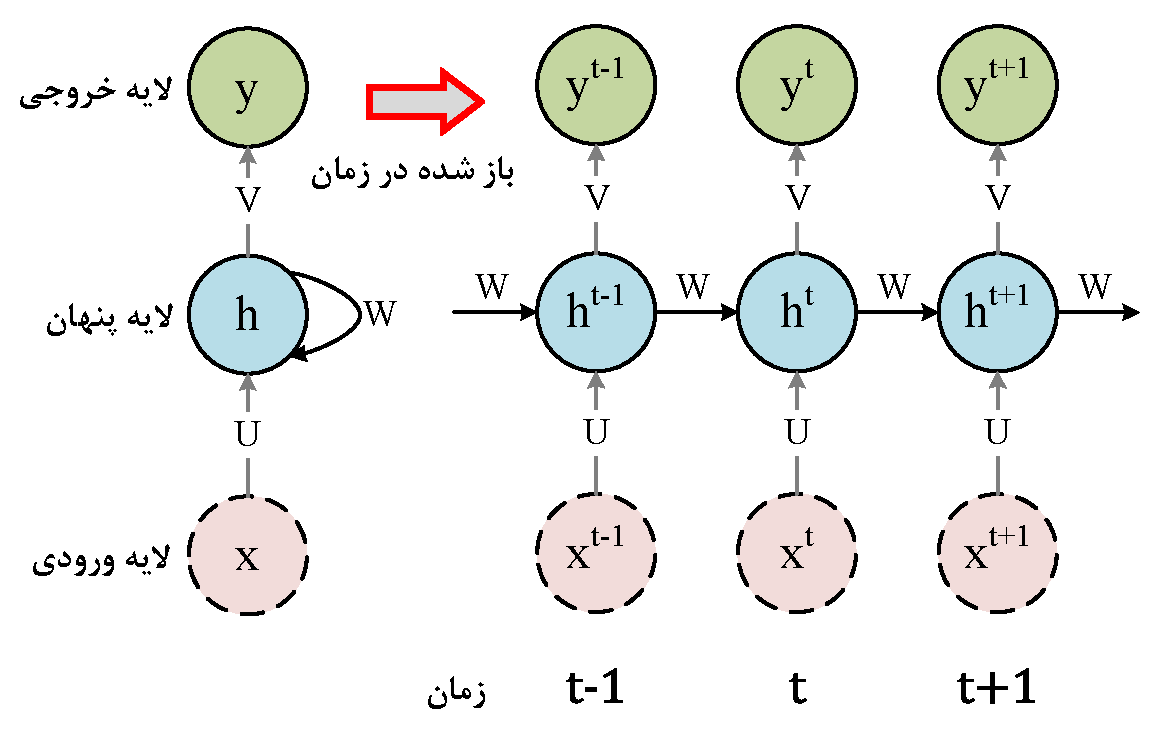
\includegraphics[width=0.8\textwidth, clip=true,  trim= 0 0 0 0]{chapter2/ch2_rnn_crop.pdf}
 	%\includegraphics[width=\textwidth]{figs/chapter1/ch1_fuzz_testing_flowchart2.png}
 	\caption[گراف محاسباتی شبکه عصبی مکرر]
 	{
 		 گراف محاسباتی مربوط به یک شبکه عصبی مکرر با یک لایه پنهان که یک توالی ورودی از مقادیر 
 		 $ x = <x^{(1)}, x^{(2)}, x^{(3)}, ..., x^{(n)}> $
 		 را به یک توالی خروجی از مقادیر 
 		 $ y = <y^{(1)}, y^{(2)}, y^{(3)}, ..., y^{(n)}> $
 		 نگاشت می‌کند. فرض شده است که خروجی $ y $ احتمال‌های نرمال نشده است، بنابراین خروجی نهایی شبکه یعنی $ \hat{y} $ از اعمال تابع بیشینه هموار روی $ y $  حاصل می‌شود. چپ: شبکه عصبی مکرر به‌صورت یال بازگشتی (گراف جهت‌دار دارای دور). راست: همان شبکه به‌صورت باز شده در زمان، به نحوی که هر گره با برچسب مرحله زمانی مشخص شده است \cite{Goodfellow-et-al-2016}.
 	}
 	\label{ch2_rnn.pdf}
 	%\ref{ch2_rnn.pdf}
 \end{figure}
 
 
 
 در ‏شکل \ref{ch2_rnn.pdf}، \gls{RNN} با یک لایه پنهان نشان داده شده است. اما می‌توان \gls{RNN}ژرف با چندین لایه پنهان نیز داشت. همچنین طول توالی‌‌های ورودی و خروجی می‌تواند بسته به مسئله مورد نظر متفاوت باشد. کارپتی\LTRfootnote{A. Karpathy (\href{http://karpathy.github.io/}{http://karpathy.github.io/})}
 	\cite{Karpathy2016}
  \gls{RNN}ها را از منظـر طول توالی ورودی و طول توالی خروجی به چند دسته تقسیم‌بندی کرده است. شکل \ref{ch2_karpathy_rnn_crop.pdf} این دسته‌بندی را نشان می‌دهد.
 
 
 \begin{figure}%[ht!]%[tbh!]%[ht]%[t!]
 	\centering
 	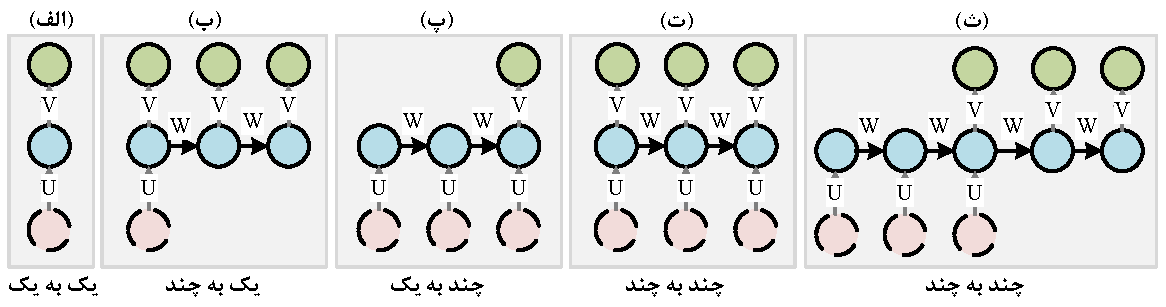
\includegraphics[width=1.0\textwidth, clip=true,  trim= 0 0 0 0]{chapter2/ch2_rnn_karpathy_crop.pdf}
 	%\includegraphics[width=\textwidth]{figs/chapter1/ch1_fuzz_testing_flowchart2.png}
 	\caption[انواع مختلف شبکه عصبی مکرر بر اساس طول توالی ورودی و خروجی]
 	{
 طرح‌واره‌ای از انواع حالت‌های مختلف شبکه عصبی مکرر براساس طول توالی ورودی و طول توالی خروجی. (الف): شبکه عصبی استاندارد، (ب): شبکه یک به چند، (پ): شبکه چند به یک، (ت) و (ث): شبکه‌های چند به چند \cite{Karpathy2016}. 
 	}
 	\label{ch2_karpathy_rnn_crop.pdf}
 	%\ref{ch2_karpathy_rnn_crop.pdf}
 \end{figure}
 
 
 
 \subsubsection{آموزش شبکه عصبی مکرر}
 الگوریتم پس‌انتشار برای آموزش \gls{RNN} هم قابل استفاده است. در واقع \gls{RNN} همان شبکه عصبی روبه‌جلو است که یک بازخورد از وزن‌‌های \gls{TimeStep} قبل دارد. در نتیجه خطا هنوز به‌صورت روی‌به‌عقب از \gls{TimeStep}  $ t $ منتشر می‌شود. بسته به طول توالی ورودی و میزان منابع محاسباتی این انتشار تا \gls{TimeStep}  $ t=1 $ ادامه می‌یابد یا تحت محدودیت تعداد مشخصی \gls{Step} متوقف می‌شود. نسخه‌ای از الگوریتم پس‌انتشار که می‌تواند به‌کل طول توالی ورودی اعمال شود، پس‌انتشار در زمان (\gls{BPTT}) نام دارد. محدودیت منابع محاسباتی ایجاب می‌نماید که طول توالی ورودی مقدار مشخصی قرار داده شود یا پس‌انتشار در تعداد محدودی گام‌زمانی متوقف شود \cite{Goodfellow-et-al-2016}.  
 
 
 \subsubsection{حافظه کوتاه‌مدت بلند}
 \gls{RNN} در حالت استاندارد، برای توالی‌‌های طولانی که وابستگی بین ورودی‌هایی با فاصله زیاد وجود دارد، قادر به حفظ این وابستگی‌ها نیست؛ به‌بیان دیگر گرادیان در دوره‌‌های زمانی بلند مدت تمایل به \gls{Vanishing} یا \gls{Explosion} (زیاد شدن بی‌اندازه) دارد. در حالت ناپدید شدن گرادیان، یادگیری مدل متوقف می‌شود. مدل حافظه کوتاه‌مدت بلند (\gls{LSTM})  برای مقابله با مسئله بالا و افزایش قدرت به‌خاطر‌سپاری   \gls{RNN} ایجاد شده است. هسته این مدل سلول حافظه C است که در آن بر خلاف شبکه مکرر استاندارد که خروجی هر واحد تنها با اعمال یک تابع انگیزش ایجاد می‌شود، خروجی با محاسبات پیچیده‌تری تعیین می‌شود که به‌ویژه هدف آنها منظم‌سازی و حفظ قدرت گرادیان است. ایده اصلی در \gls{LSTM} تخصیص مسیری مجزا علاوه بر یال بازخوردی حالت پنهان، برای جریان حافظه است.
 
 جزئیات عملکرد \gls{LSTM} در \cite{Goodfellow-et-al-2016} توضیح داده شده است. امروزه به‌طور پیشفرض از \gls{LSTM} در پیاده‌سازی \gls{RNN} استفاده می‌شود \cite{DBLP:journals/corr/GreffSKSS15}. البته راه‌کارهای جایگزین دیگری مشابه \gls{LSTM}، نیز مطرح شده‌اند مانند \gls{GRU} \cite{DBLP:journals/corr/ChoMGBSB14}، اما عملکرد آنها بهتر از  \gls{LSTM} نیست. مطالعه جامعی روی \gls{RNN} و انواع آن برای یادگیری توالی‌ها در \cite{DBLP:journals/corr/Lipton15} انجام شده است. کلیه مدل‌های یادگیری ژرف معرفی شده در این پایان‌نامه از \gls{LSTM} در هسته خود استفاده می‌کنند. 
 
 
 
 
 
 
 \section{مدل زبانی}\label{sec:language_model}
 در فصل 
 \ref{chapter1}
 به استفاده از \gls{LM} در روش پیشنهادی خود، اشاره کردیم. 
 \gls{LM} 
 یک مفهوم پایه در \gls{NLP} است که امکان پیش‌بینی نشانه بعدی در یک توالی را فراهم می‌کند. به‌بیان دقیق‌تر \gls{LM} عبارت است از یک توزیع احتمالی روی یک توالی از نشانه‌ها (اغلب واژه‌ها) که احتمال وقوع یک توالی داده شده را مشخص می‌کند. در نتیجه می‌توان بین چندین توالی داده شده برای مثال چند جمله، آن را که محتمل‌تر است، انتخاب کرد. 
 \gls{LM}  
 برای توالی 
 $ x = <x^{(1)}, x^{(2)}, x^{(3)}, ..., x^{(n)}> $
 به‌صورت زیر تعریف می‌شود\cite{Luong2016}:
 \begin{equation}\label{languagemodelformula}
 	p(x) = \prod_{t=1}^{n}p(x^{(t)}|x^{ <t})
 \end{equation} 
 
 
 در رابطه \ref{languagemodelformula} هر جمله منفرد 
 $ p(x^{(t)}|x^{ <t}) $
 احتمال شرطی نشانه 
 $ x^{(t)} $
 به شرط وقوع (ظاهر شدن) $ t $ نشانه قبلی  $ x^{ <t} $ در توالی است که به آن \gls{Context} یا \gls{History} نیز می‌گویند. در عمل محاسبه این احتمال به‌صورت رابطه \ref{languagemodelformula} تقریباً غیر ممکن است؛ زیرا، نیازمند داشتن همه تـوالی‌های ممکن هستیم. مدل‌های سنـتی \lr{n-gram} برای غلبه بر چالش‌های محاسباتی، با استفاده از فرض مارکوف رابطه \ref{languagemodelformula} را به درنظر گرفتن تنها $ n-1 $ نشانه قبلی محدود می‌کنند. اگرچه در بسیاری از مسائل این مدل‌ها به خوبی پاسخ‌گو هستند؛ اما، برای توالی‌های طولانی (بیشتر از 4 یا 5 نشانه) و نیز مشاهده نشده مناسب نیستند. در حالتی که نشانه فعلی پیش‌ از این مشاهده نشده باشد، احتمال صفر به آن نسبت داده می‌شود که سبب صفر شدن احتمال پایانی می‌گردد. برای حل این مشکل، مدل‌های \lr{n-gram} نیازمند اعمال فنون \gls{Smoothing} هستند \cite{Jurafsky2017}. این فنون، راه‌حل‌هایی برای از بین بردن احتمال‌های صفر پیشنهاد می‌دهند. در هر صورت، مدل‌های \lr{n-gram} با محدودیت‌های جدی روبه‌رو هستند.


 
\subsection{مدل زبانی عصبی}
  می‌توان از \gls{RNN} برای ایجاد مدل زبانی استفاده کرد. این مدل‌ها را مدل زبانی عصبی (\gls{NLM}) می‌گویند. استفاده از \gls{RNN} هر دو مشکل اشاره شده در بالا را برطرف می‌کند. یعنی هم امکان پیش‌بینی توالی‌های طولانی‌تر فراهم می‌شود و هم وقوع احتمالات صفر از بین می‌رود \cite{Luong2016}.  شکل \ref{ch2_nlm_persian_crop.pdf} یک معماری از \gls{RNN} برای ساخت مدل زبانی در \gls{NLP} را نشان می‌دهد. چون هدف مدل زبانی پیش‌بینی نشانه بعدی است، توالی $ x $  را در ورودی شبکه قرار داده و خروجی متناظر با آن را همان توالی $ x $ که یک واحد روبه‌جلو شیفت داده شده است، می‌گذارند. این روش آموزش شبکه \lr{Teacher Forcing} می‌گویند \cite{Goodfellow-et-al-2016}.
  
  \begin{figure}%[ht!]%[tbh!]%[ht]%[t!]
  	\centering
  	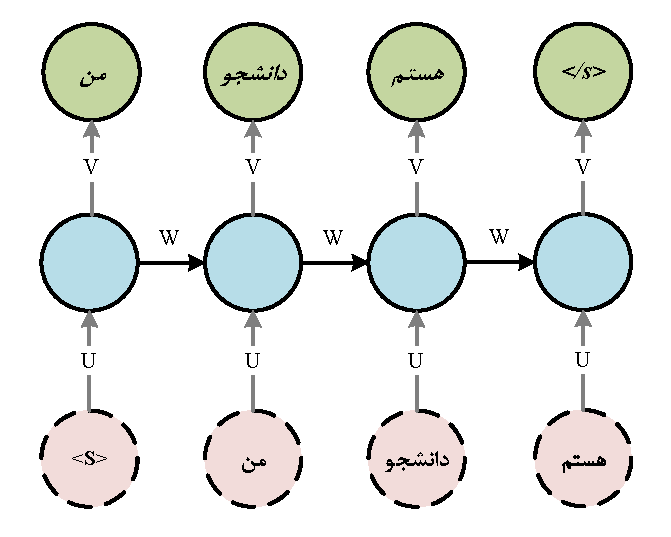
\includegraphics[width=0.7\textwidth, clip=true,  trim= 0 0 0 0]{chapter2/ch2_nlm_persian_crop.pdf}
  	%\includegraphics[width=\textwidth]{figs/chapter1/ch1_fuzz_testing_flowchart2.png}
  	\caption[مدل زبانی عصبی مکرر]
  	{
  		طرح‌واره‌ای از معماری یک مدل زبانی ایجاد شده با استفاده از \gls{RNN}. $ <s> $ نشانه شروع توالی و $ </s> $ نشانه خاتمه توالی در ابتدا و انتهای هر توالی موجود در مجموعه آموزش قرار داده می‌شود. بدین ترتیب، تولید توالی جدید پس از پیش‌بینی نشانه پایان، متوقف می‌گردد \cite{Luong2016}.
  	}
  	\label{ch2_nlm_persian_crop.pdf}
  	%\ref{ch2_nlm_persian_crop.pdf}
  \end{figure}
  
  
  مدل‌های زبانی را \gls{GenerativeModel} نیز می‌نامند؛ زیرا یک توزیع احتمالی روی توالی‌های یک زبان می‌دهند که با نمونه‌‌برداری از آن می‌توان توالی‌های جدید تولید کرد. در \gls{NLP} نشانه‌های هر توالی واژه‌ها هستند، اما می‌توان این مدل را در سطح کاراکتر نیز آموزش داد. ایده اصلی در این پایان‌نامه نیز همین است. هر فایل زبان و قواعد مخصوص به خود را دارد که در مشخصه‌های قالب فایل ذکر شده است. با ایجاد یک مدل زبانی برای این زبان در سطح کاراکتر،  امکان پیش‌بینی نشانه بعدی از روی یک توالی از نشانه‌های داده شده فراهم می‌شود. با نمونه برداری از این مدل زبانی می‌توان داده‌های آزمون جدیدی ایجاد کرد.
 
 \subsection{ارزیابی مدل زبانی}
 چگونه می‌توان میزان خوب بودن یک مدل زبانی را تعیین کرد؟ یک روش برای ارزیابی مدل زبانی، قرار دادن آن در یک وظیفه مشخص و اندازه‌گیری میزان دقت نتایج حاصله است. به این روش‌ \gls{ExtrinsicEvaluation} می‌گویند
 \cite{Jurafsky2017}.
  برای مثال در یک وظیفه تصحیح خودکار غلط‌های املایی، تعداد واژه‌های نادرستی که به‌درستی با واژه‌های صحیح جایگزین شده‌اند را شمارش می‌کنیم و بر تعداد کل واژه‌های غلط تقسیم می‌نماییم. ارزیابی بیرونی، زمان‌بر، پرهزینه و مختص به وظیفه اجرا شده خواهد بود.  روش دیگر استفاده از \gls{IntrinsicEvaluation} است \cite{Jurafsky2017}. معیار \gls{Perplexity} با هدف ارزیابی  درونی مدل زبانی، به‌صورت زیر تعریف می‌شود \cite{mikolov2012statistical}:
  
 \begin{equation}\label{ppl}
 \begin{split}
 	PP_{LM}(x) & = \sqrt[n]{\prod_{i=1}^n(\frac{1}{p(x^{(i)}|<x^{(1)}, ..., x^{(i-1)}>)}} \\
 	& = 2^{-\frac{1}{n}\sum_{i=1}^n\log_{2}{p(x^{(i)}|<x^{(1)}, ..., x^{(i-1)>})}}
 \end{split}
 \end{equation}
در رابطه 
\ref{ppl}،
$ x $
 توالی مورد ارزیابی است. همان‌طور که مشاهده می‌شود \gls{Perplexity} در ارتباط مستقیم با \gls{CrossEntropyError} (رابطه \ref{CrossEntropyLossFunction}) است که میزان اختلاف بین مدل و نمونه‌های مجموعه آزمون را نشان می‌دهد. بنابراین هرچه‌قدر میزان سرگشتگی پایین‌تر باشد، مدل زبانی بهتر است. پایه توان و پایه لـــگاریتم در رابطه \ref{ppl} می‌تواند مقادیری به‌غیر از 2 انتخاب شود. اما در هر حالت هر دو پایه بایستی یکسان باشند تا تساوی اول (بالا) و دوم (پایین) رابطه برقرار گردد. معمولاً از پایه لگاریتم طبیعی در این رابطه استفاده می‌شود 
\cite{DBLP:journals/corr/AbadiABBCCCDDDG16}.

برای درک بهتر نحوه ارزیابی توسط این معیار، توالی 
$ x = <x^{(1)}, x^{(2)}, x^{(3)}, ..., x^{(n)}> $
را در نظر می‌گیریم که متشکل از $ V $ نشانه متفاوت است. $ V $ مجموعه \gls{Vocabulary} زبان است. در غیاب مدل زبانی (بدترین حالت)، تنها می‌توانیم ادعا کنیم که هر نشانه دست‌کم با احتمال 
$ \frac{1}{V} $
در توالی رخ می‌دهد (\gls{BranchingFactor}). بدیهی است که این احتمال برای همه نشانه‌ها یکسان است. برای توالی $ x $ پس از جایگزینی احتمال آن در رابطه  \ref{ppl} داریم:
\begin{equation*}
PP_{LM}(x) = \sqrt[n]{\prod_{i=1}^n(\frac{1}{\frac{1}{V}})} = \sqrt[n]{V^{n}} = V
\end{equation*} 
 بنابراین در بدترین حالت میزان سرگشتگی برابر با اندازه مجموعه \gls{Vocabulary} زبان است. حال چنان‌چه از مدل زبانی استفاده کنیم، احتمال نسبت داده شده به وقوع هر نشانه، نسبت به حالت عدم استفاده از مدل زبانی، افزایش و در نتیجه سرگشتگی کاهش خواهد یافت. در ارزیابی مدل‌های این پایان‌نامه از معیار سرگشتگی استفاده می‌کنیم. 
 
 
 
 
 
 
 \section{خلاصه}
 در این فصل مفاهیم اولیه سه حوزه کلی مطرح در این پایان‌نامه یعنی آزمون نرم‌افزار، آزمون فازی و یادگیری ژرف را بیان کردیم. آزمون نرم‌افزار به‌عنوان یک مسئله تصمیم‌ناپذیر تعریف گردید و معیارهای پوشش برای ارزیابی آن معرفی شدند. آزمون فازی به عنوان یک فن مطرح در آزمون نرم‌افزار، معرفی و از سه دیدگاه مختلف مورد طبقه‌بندی و بحث قرار گرفت: نخست، از دیدگاه اطلاعات در دسترس از \gls{SUT} به سه دسته آزمون جعبه سیاه، جعبه سفید و جعبه خاکستری تقسیم گردید. دوم، از دیدگاه روش‌های تولید داده آزمون به سه دسته مبتنی بر جابه‌جایی، مبتنی بر تولید و نیز ترکیبی تقسیم‌بندی شد. سوم، با توجه به دریافت بازخورد از نتیجه اجرا به دو دسته دارای بازخورد و بدون بازخورد تفکیک گشت. ابزار خودکارسازی آزمون فازی تحت عنوان کلی فازر معرفی و معماری آن تشریح شد.  فازرها با توجه به طبقه‌بندی‌های فوق در بحث آزمون فازی و نیز با توجه به نوع ورودی \gls{SUT} متفاوت هستند. فازرهای قالب فایل مربوط به برنامه‌هایی با ورودی فایل هستند. برای اطلاعات بیشتر در زمینه آزمون نرم‌افزار خواننده را به
  \cite{ammann2016introduction, PaulC.Jorgensen2014} 
 ارجاع می‌دهیم. در زمینه آزمون فازی نیز خواننده را به
 \cite{Chen2018, Mcnally2012, Sutton:2007:FBF:1324770}      
 رجوع می‌دهیم.
 
 در بخش پایانی این فصل، یادگیری ژرف به عنوان زیرشاخه‌ای از یادگیری ماشینی با استفاده از شبکه‌های عصبی مصنوعی، تفهیم شد. شبکه عصبی مورد استفاده در یادگیری ژرف را شبکه عصبی ژرف گویند. \gls{RNN} نوع خاصی از شبکه‌های عصبی ژرف است که برای پردازش وظیفه‌های مبتنی بر توالی مثل مدل زبانی استفاده می‌شود. ساختار یک قالب فایل زبان مختص به خود را دارد و هدف از مطرح کردن اصول اولیه یادگیری ژرف استفاده از مدل‌های این فن، در یادگیری ساختار فایل، جهت تولید داده آزمون جدید است که در فصل 4 به آن خواهیم پرداخت. الگوریتم‌های آموزش شبکه‌های عصبی ژرف ریاضیات گسترده‌ای دارد که به‌طور خلاصه به موارد مهم آن اشاره شد. جهت مطالعه مبسوط این الگوریتم‌ها خواننده را به
 \cite{Goodfellow-et-al-2016}
 ارجاع می‌دهیم. همچنین توضیح کاملی از روش‌های یادگیری توالی با استفاده از \gls{RNN}ها در 
 \cite{DBLP:journals/corr/Lipton15}
 آمده است. در فصل بعد برخی از تازه‌ترین کارهای مرتبط با مفاهیم مطرح شده در این فصل توضیح داده می‌شوند.   
 
 
 
 
 
 
 